% !TeX program = xelatex
% !TeX encoding = UTF-8
\documentclass[UTF8,a4paper,zihao=-4,fontset=none]{ctexart}
\usepackage[left=25mm,right=25mm,top=22mm,bottom=22mm]{geometry}
\usepackage{amsmath,amssymb,graphicx,booktabs,tabularx,array,makecell}
\usepackage{caption,subcaption,placeins,fancyhdr,enumitem,fvextra}
\usepackage{newtxmath}
\usepackage{tocloft}
\usepackage{needspace}
\usepackage[hidelinks,unicode]{hyperref}
\setmainfont{Times New Roman}
\setsansfont{Times New Roman}
\setmonofont{Times New Roman}
\setmathrm{Times New Roman}
\setboldmathrm{Times New Roman Bold}
\DeclareSymbolFont{operators}{TU}{\rmdefault}{m}{n}
\SetSymbolFont{operators}{bold}{TU}{\rmdefault}{b}{n}
\setCJKmainfont{SimSun}[AutoFakeBold=2,ItalicFont=SimSun]
\setCJKsansfont{SimHei}[AutoFakeBold=2]
\setCJKmonofont{SimSun}
\setCJKfamilyfont{zhsong}{SimSun}[AutoFakeBold=2,ItalicFont=SimSun]
\setCJKfamilyfont{zhhei}{SimHei}[AutoFakeBold=2]
\providecommand{\songti}{\CJKfamily{zhsong}}
\providecommand{\heiti}{\CJKfamily{zhhei}}
\graphicspath{{figures/}}
\setlength{\parindent}{2em}
\setlength{\parskip}{0pt}
\linespread{1.25}
\raggedbottom
\setlength{\emergencystretch}{2em}
\ctexset{
  section={format=\heiti\zihao{4}\bfseries,number=\arabic{section},aftername={\quad},beforeskip=0pt,afterskip=0pt},
  subsection={format=\heiti\zihao{4}\mdseries,beforeskip=0pt,afterskip=0pt},
  subsubsection={format=\songti\zihao{4}\mdseries,beforeskip=0pt,afterskip=0pt}
}
\setcounter{tocdepth}{3}
\renewcommand{\cfttoctitlefont}{\heiti\zihao{4}\bfseries}
\setlength{\cftbeforetoctitleskip}{0pt}
\setlength{\cftaftertoctitleskip}{0pt}
\setlength{\cftbeforesecskip}{0pt}
\captionsetup{font=small,labelfont=bf,labelsep=quad,skip=6pt,textfont=bf}
\captionsetup[subfigure]{font=small}
\captionsetup[table]{justification=centering,singlelinecheck=false}
\setlength{\textfloatsep}{12pt plus 2pt minus 2pt}
\setlength{\floatsep}{10pt}
\setlength{\intextsep}{10pt plus 2pt minus 2pt}
\makeatletter
\setlength{\@fptop}{0pt}
\setlength{\@fpsep}{12pt}
\setlength{\@fpbot}{0pt plus 1fil}
\makeatother
\renewcommand{\topfraction}{0.92}
\renewcommand{\bottomfraction}{0.85}
\renewcommand{\textfraction}{0.08}
\renewcommand{\floatpagefraction}{0.72}
\setcounter{topnumber}{3}
\setcounter{bottomnumber}{3}
\setcounter{totalnumber}{5}
\pagestyle{fancy}
\fancyhf{}
\fancyfoot[C]{\small\thepage}
\setlength{\headheight}{15pt}
\renewcommand{\headrulewidth}{0pt}
\newcolumntype{Y}{>{\centering\arraybackslash}X}
\renewcommand{\tabularxcolumn}[1]{m{#1}}
\newcommand{\ReportTableHead}[1]{\textbf{#1}}
\DefineVerbatimEnvironment{Code}{Verbatim}{fontsize=\small,frame=single,breaklines=true,samepage=true,framesep=5pt}
\newcommand{\shot}[4][\linewidth]{%
  \begin{figure}[htbp]
    \centering
    \includegraphics[width=#1,height=0.69\textheight,keepaspectratio]{#2}
    \caption{#3}\label{#4}
  \end{figure}
}
\hypersetup{pdftitle={实验2：词向量的学习与分析},pdfsubject={自然语言处理课程实验报告}}

\begin{document}
\pagestyle{plain}
\begin{center}
  {\heiti\zihao{3}\bfseries 实验二：词向量的学习与分析\par}
\end{center}
\tableofcontents
\clearpage
\pagestyle{fancy}

\section{实验目的}

本实验通过独热表示、基于共现统计的低维表示和 Skip-gram 模型，了解词语如何转换为数值向量，以及词向量与上下文之间的关系。实验内容和语料以教师提供的实验设计为依据\cite{lab}。

具体目的包括：理解独热表示的局限性；根据上下文窗口构造训练样本；使用 PyTorch 实现并训练小型 Skip-gram 模型；通过余弦相似度查询相似词；分析语料、窗口和降维对结果的影响。同时，通过构造 CBOW 样本以及比较 Word2Vec、GloVe 和 ELMo，理解不同词表示方法的基本区别。

\section{实验环境}

实验在 Windows 系统下进行，使用 Anaconda 管理 Python 环境，在 Jupyter Notebook 中编写和运行代码。最终使用的内核为“Python（NLP实验2）”，模型在 CPU 上训练。

\begin{table}[htbp]
\centering\small
\caption{实验环境与工具}\label{tab:environment}
\begin{tabularx}{\linewidth}{cY}
\toprule
\ReportTableHead{环境或工具} & \ReportTableHead{版本或用途}\\
\midrule
Python & 3.10.22\\
PyTorch & 2.14.1+cpu，用于模型建立与训练\\
NumPy & 2.2.6，用于矩阵运算和 SVD\\
pandas & 2.3.3，用于整理结果表格\\
Matplotlib & 3.10.9，用于绘制损失曲线和散点图\\
scikit-learn & 1.7.2，用于 PCA 降维\\
Jupyter Notebook & 用于代码运行与结果记录\\
\bottomrule
\end{tabularx}
\end{table}

实验语料已通过空格划分词语，因此直接使用 \texttt{split()} 得到词序列。本次没有另外进行 jieba 中文分词，也没有使用预训练词向量。

\section{独热表示与分布式表示对比}

\subsection{独热表示及其局限性}

首先选取“猫、狗、鸟、飞机”四个词，按照词表编号建立独热向量。每个词对应一个4维向量，仅自身编号对应的位置为1，其余位置为0。对于任意两个不同词，其独热向量的内积为0，欧氏距离为
\[
\sqrt{(1-0)^2+(0-1)^2}=\sqrt{2}\approx1.4142\text{。}
\]

因此，“猫—狗”和“猫—飞机”具有相同的独热距离及余弦相似度，无法体现两组词在语义或用法上的差别。独热向量的维度还会随词表规模增大，形成高维稀疏表示。

词袋表示通常用词频或词权重描述一段文本，也依赖固定词表，但它主要用于表示文本，与本实验中为单个词建立向量的任务有所不同。

\subsection{基于上下文统计的低维表示}

实验采用12条教学短语，在左右各2个词的窗口内统计目标词周围的上下文。四个目标词作为矩阵行，上下文词作为矩阵列，得到一个 $4\times14$ 的共现矩阵，构造过程和输出如图\ref{fig:original-counts}所示。

手工检查可知，“猫—可爱”的计数为1，“猫—宠物”和“狗—宠物”的计数均为1，与程序输出一致。随后，对共现矩阵逐行进行归一化，使用奇异值分解（SVD）保留前三个方向，得到 $4\times3$ 的低维词向量。

\shot{01_original_cooccurrence.png}{原始教学语料及其共现矩阵}{fig:original-counts}

\begin{figure}[htbp]
\centering
\begin{subfigure}[t]{0.46\linewidth}
\centering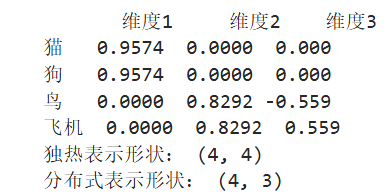
\includegraphics[width=\linewidth]{02_original_svd.png}
\caption{原始SVD词向量及表示形状}
\end{subfigure}\hfill
\begin{subfigure}[t]{0.46\linewidth}
\centering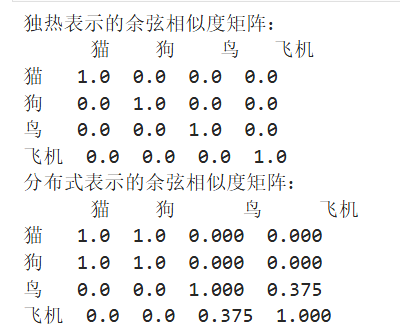
\includegraphics[width=\linewidth]{04_original_cosine_matrices.png}
\caption{两种表示的余弦相似度矩阵}
\end{subfigure}
\caption{原始语料下的低维表示与相似度矩阵}\label{fig:original-svd-matrix}
\end{figure}

原始语料下的词对指标见表\ref{tab:original-pairs}，相应运行输出见图\ref{fig:original-pairs}。

\begin{table}[htbp]
\centering\small
\caption{原始语料下独热表示与SVD表示的词对指标}\label{tab:original-pairs}
\begin{tabularx}{\linewidth}{Ycccc}
\toprule
\ReportTableHead{词对} & \ReportTableHead{\makecell{独热\\欧氏距离}} & \ReportTableHead{\makecell{独热\\余弦相似度}} & \ReportTableHead{\makecell{SVD\\欧氏距离}} & \ReportTableHead{\makecell{SVD\\余弦相似度}}\\
\midrule
猫—狗 & 1.4142 & 0.0000 & 0.0000 & 1.0000\\
猫—鸟 & 1.4142 & 0.0000 & 1.3844 & 0.0000\\
猫—飞机 & 1.4142 & 0.0000 & 1.3844 & 0.0000\\
狗—鸟 & 1.4142 & 0.0000 & 1.3844 & 0.0000\\
狗—飞机 & 1.4142 & 0.0000 & 1.3844 & 0.0000\\
鸟—飞机 & 1.4142 & 0.0000 & 1.1180 & 0.3750\\
\bottomrule
\end{tabularx}
\end{table}

\shot{03_original_pair_metrics.png}{原始语料下六组词对的指标输出}{fig:original-pairs}

原始短语中，“猫”和“狗”共享“可爱、宠物、家中、陪伴、吃”等上下文，因此具有相近的上下文分布。它们在“鱼”和“肉”列仍有差别，但截断为3维后，区分这部分差异的方向没有被保留，最终向量重合。这不意味着两个词完全同义。

“鸟”和“飞机”共享“天空、空中、移动”等上下文，因此相似度高于部分其他词对，但二者分别属于动物和交通工具，也不是同义词。

本步骤用于演示上下文统计如何形成低维表示，并非 Word2Vec 或 GloVe 的实现。向量的各个维度也不能直接命名为“动物性”“飞行性”等语义属性。

\subsection{修改语料前后的比较}

按照实验要求，将一条关于“狗”的短语由“可爱 狗 宠物”替换为“狗 天空 飞行”。其他短语、窗口大小和 SVD 保留维数不变，再重新统计共现矩阵、计算词向量及相似度。整个过程中只修改输入语料，没有直接修改向量数值。

\shot{05_modified_cooccurrence.png}{将一条“狗”的短语改为飞行相关短语后重新统计共现矩阵}{fig:modified-counts}

\begin{figure}[htbp]
\centering
\begin{subfigure}[t]{0.47\linewidth}
\centering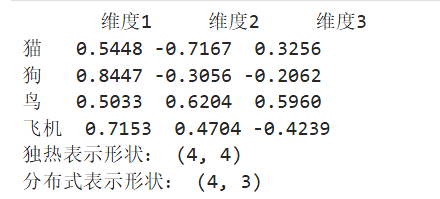
\includegraphics[width=\linewidth]{06_modified_svd.png}
\caption{修改后的SVD词向量}
\end{subfigure}\hfill
\begin{subfigure}[t]{0.47\linewidth}
\centering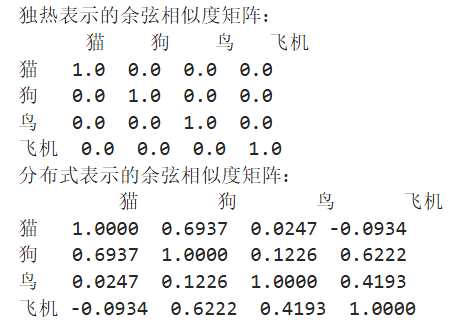
\includegraphics[width=\linewidth]{08_modified_cosine_matrices.png}
\caption{修改后的余弦相似度矩阵}
\end{subfigure}
\caption{修改语料后重新计算的词向量与相似度矩阵}\label{fig:modified-svd-matrix}
\end{figure}

\shot{07_modified_pair_metrics.png}{修改语料后的六组词对指标输出}{fig:modified-pairs}

\begin{table}[htbp]
\centering\small
\caption{修改语料前后的SVD余弦相似度比较}\label{tab:modification}
\begin{tabularx}{\linewidth}{Ycc}
\toprule
\ReportTableHead{词对} & \ReportTableHead{修改前余弦相似度} & \ReportTableHead{修改后余弦相似度}\\
\midrule
猫—狗 & 1.0000 & 0.6937\\
猫—鸟 & 0.0000 & 0.0247\\
猫—飞机 & 0.0000 & $-0.0934$\\
狗—鸟 & 0.0000 & 0.1226\\
狗—飞机 & 0.0000 & 0.6222\\
鸟—飞机 & 0.3750 & 0.4193\\
\bottomrule
\end{tabularx}
\end{table}

修改后，“狗”在“可爱”和“宠物”列的计数由1变为0，在“天空”和“飞行”列的计数由0变为1。“猫—狗”的余弦相似度下降约0.3063，而“狗—飞机”的相似度上升。

这一结果说明，基于上下文统计得到的词表示会随语料变化。由于 SVD 对整个矩阵进行分解，修改一行还可能影响其他词的低维表示。该实验使用经过设计的短语语料，只能说明当前统计关系，不能证明词向量在真实语言应用中的可靠性。

\FloatBarrier
\section{Skip-gram训练样本构造}

\subsection{准备语料与建立词表}

Skip-gram 实验使用8个句子，例如“猫 喜欢 吃 鱼”“狗 喜欢 吃 肉”“飞机 在 天空 飞行”等。语料共包含37个词次，去重后得到23个词。

使用 \texttt{Counter} 统计词频，根据词频建立词表，再构造词语与编号之间的双向映射。训练时使用词编号作为模型输入，输出检查时再将编号转换为词语。准备语料与建立词表的实际运行记录见图\ref{fig:corpus-vocabulary}。

这里的语料与任务1的12条短语不同。修改任务1中关于“狗”的短语，没有改变 Skip-gram 的这8个训练句子。

\begin{figure}[htbp]
\centering
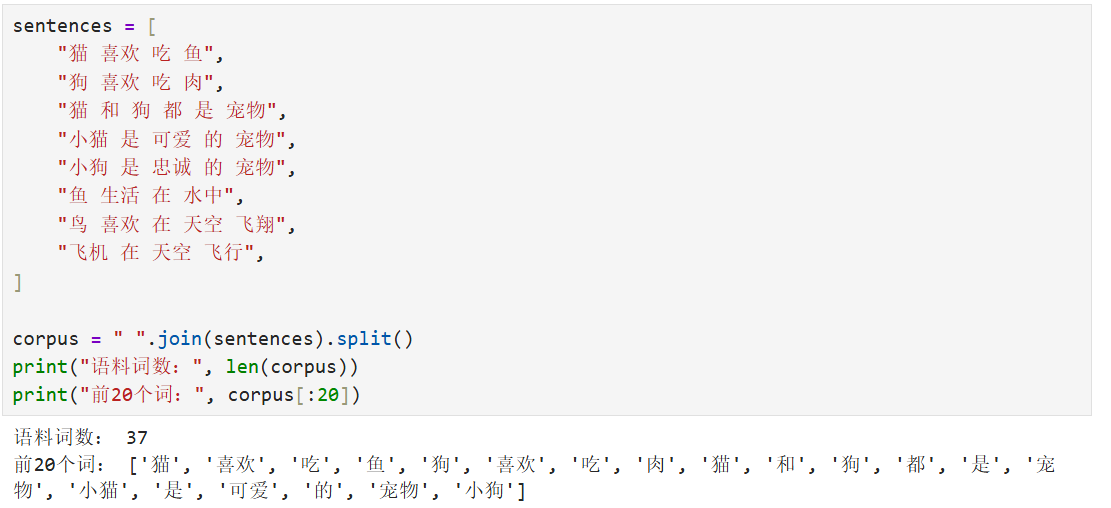
\includegraphics[width=\linewidth]{09_training_corpus.png}\par\vspace{5pt}
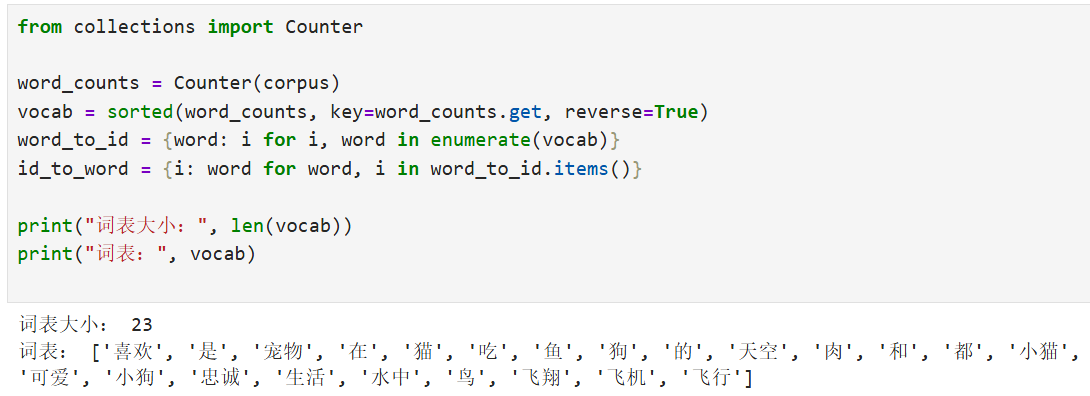
\includegraphics[width=\linewidth]{10_vocabulary.png}
\caption{Skip-gram训练语料与23词词表的构建结果}\label{fig:corpus-vocabulary}
\end{figure}

\Needspace{12\baselineskip}
\subsection{构造中心词—上下文词样本}

Skip-gram 的任务是给定中心词，预测窗口内的上下文词。窗口大小为1表示分别查看中心词左侧和右侧最多一个词。对于“猫 喜欢 吃 鱼”，可以生成以下6个样本：

\noindent\begin{minipage}{\linewidth}
\begin{Code}
猫 -> 喜欢
喜欢 -> 猫
喜欢 -> 吃
吃 -> 喜欢
吃 -> 鱼
鱼 -> 吃
\end{Code}
\end{minipage}

程序对每个句子分别遍历，跳过中心词自身，将中心词编号和上下文词编号保存为一个训练样本。原始语料在窗口大小为1时共生成58个样本，见图\ref{fig:skipgram-samples}。中心词张量和上下文词张量的形状均为 \texttt{torch.Size([58])}，分别作为模型输入和目标标签。

\shot{11_skipgram_samples.png}{Skip-gram样本构造函数与前十个训练样本}{fig:skipgram-samples}

\subsection{不同窗口大小的比较}

\begin{table}[htbp]
\centering\small
\caption{不同上下文窗口对应的样本数量}\label{tab:windows}
\begin{tabular}{cc}
\toprule
\ReportTableHead{窗口大小} & \ReportTableHead{训练样本数}\\
\midrule
1 & 58\\
2 & 100\\
3 & 126\\
\bottomrule
\end{tabular}
\end{table}

\shot{12_window_comparison.png}{窗口大小为1、2、3时的样本数量输出}{fig:windows}

窗口增大后，每个中心词能够关联更远的上下文词，因此样本数量增加。较小窗口主要反映近邻搭配；较大窗口可以纳入更宽范围的信息，但也可能包含与中心词关系较弱的词。窗口选择应结合语料和任务目的。

如果将全部句子拼接后直接构造窗口，前一句末尾的词可能与后一句开头的词形成不合理的训练关系。本实验逐句构造样本，避免了跨句子边界的问题。本次只比较了三个窗口下的样本数量，实际模型使用窗口大小1，没有分别训练三个窗口模型。

\subsection{提高任务：构造CBOW样本}

连续词袋模型（CBOW）使用上下文词预测中心词，与 Skip-gram 的预测方向相反。例如，中心词为“喜欢”时，可以生成 $[\text{猫},\text{吃}]\to\text{喜欢}$。

在样本构造函数中，先收集当前中心词周围的上下文编号，再与中心词编号组成一个样本，即 \verb|(context_word_ids, center_word_id)|。

窗口大小为1时，原始语料共生成37个 CBOW 样本。句首和句尾的上下文列表可能只有一个词，句中则通常有两个词。修改后的函数与样本输出如图\ref{fig:cbow-samples}所示。

\shot{18_cbow_samples.png}{CBOW样本构造函数及其37个样本中的前十项}{fig:cbow-samples}

如果进一步建立 CBOW 模型，可以对多个上下文词向量求和或取平均，形成用于预测中心词的输入表示。本次提高任务完成了样本构造，没有进行 CBOW 模型训练，因此不能据此比较两种模型的损失或词向量质量。

在小语料中，两种方法都受到上下文不足和低频词样本较少的影响；扩大语料后，可以进一步比较训练时间、相似词结果和不同词频下的表现。

\FloatBarrier
\section{模型结构与训练过程}

\subsection{Skip-gram模型结构}

使用 PyTorch 建立由 Embedding 层和线性输出层组成的 Skip-gram 模型。Embedding 层根据中心词编号，从词向量矩阵中查找对应的10维向量。线性层再将这个向量映射为23个输出分数，对应词表中的23个候选上下文词。

模型流程为
\[
\text{中心词编号}\to\text{Embedding查表}\to\text{10维词向量}\to\text{线性层}\to\text{上下文词预测。}
\]

Embedding 参数矩阵的形状为 $23\times10$。模型返回未经归一化的输出分数，交叉熵损失函数完成对应的概率计算和损失计算，因此没有在模型中额外添加 Softmax。

\subsection{训练设置}

\begin{table}[htbp]
\centering\small
\caption{Skip-gram模型的训练参数}\label{tab:parameters}
\begin{tabularx}{\linewidth}{cY}
\toprule
\ReportTableHead{参数} & \ReportTableHead{设置}\\
\midrule
词表大小 & 23\\
词向量维度 & 10\\
上下文窗口 & 左右各1个词\\
训练样本数 & 58\\
随机种子 & 42\\
优化器 & Adam\\
学习率 & 0.03\\
损失函数 & CrossEntropyLoss\\
训练轮数 & 1000\\
输出方式 & 完整Softmax\\
每轮训练方式 & 使用全部58个样本\\
\bottomrule
\end{tabularx}
\end{table}

每轮训练依次进行梯度清零、前向计算、损失计算、反向传播和参数更新，并保存损失值。每200轮输出一次训练日志。

\subsection{训练结果}

\begin{table}[htbp]
\centering\small
\caption{训练过程中每200轮记录的损失}\label{tab:loss}
\begin{tabular}{cc}
\toprule
\ReportTableHead{训练轮数} & \ReportTableHead{损失}\\
\midrule
200 & 0.9814\\
400 & 0.9808\\
600 & 0.9806\\
800 & 0.9805\\
1000 & 0.9805\\
\bottomrule
\end{tabular}
\end{table}

损失曲线在训练初期快速下降，随后逐渐稳定。到第1000轮时，损失约为0.9805，说明模型在当前训练语料上已经趋于收敛。

\shot[0.9\linewidth]{13_training_loss.png}{Skip-gram模型训练1000轮的损失曲线}{fig:loss}

损失没有降为0并不意味着训练失败。同一个中心词可能对应多个上下文词，模型需要学习这些目标的概率分布。损失下降表明模型拟合了部分上下文关系，但还不能说明词向量具有可靠的通用语义能力。

\FloatBarrier
\section{词向量相似度结果}

\subsection{词对余弦相似度}

训练完成后，提取 Embedding 层参数，得到形状为 \texttt{torch.Size([23, 10])} 的词向量矩阵。使用余弦相似度比较词向量方向：
\[
\operatorname{cos}(a,b)=\frac{a^{\mathrm T}b}{\|a\|_2\|b\|_2}\text{。}
\]

四组词对的结果如表\ref{tab:cosine}所示，提取词向量与计算相似度的运行记录见图\ref{fig:cosine}。

\begin{table}[htbp]
\centering\small
\caption{四组词对的Skip-gram余弦相似度}\label{tab:cosine}
\begin{tabular}{cc}
\toprule
\ReportTableHead{词对} & \ReportTableHead{余弦相似度}\\
\midrule
猫—狗 & 0.7484\\
天空—飞机 & 0.5342\\
猫—飞机 & 0.3546\\
鱼—水中 & $-0.3721$\\
\bottomrule
\end{tabular}
\end{table}

\shot[0.96\linewidth]{14_embedding_similarity.png}{词向量矩阵提取与四组词对的余弦相似度计算}{fig:cosine}

在本次结果中，“猫—狗”的相似度高于“猫—飞机”，符合“猫”和“狗”具有部分相似上下文的情况。“鱼—水中”的结果为负，说明现实中的关联不一定直接表现为当前模型中较高的余弦相似度。

\subsection{相似词查询结果}

对所有词向量计算与查询词的余弦相似度，按相似度降序排列，排除查询词自身，保留前5个结果。

\begin{table}[htbp]
\centering\small
\caption{四个查询词的前五个相似词}\label{tab:nearest}
\begin{tabularx}{\linewidth}{cY}
\toprule
\ReportTableHead{查询词} & \ReportTableHead{前5个相似词及相似度}\\
\midrule
猫 & 狗0.7484、鸟0.4791、在0.4497、飞翔0.3977、飞行0.3627\\
狗 & 猫0.7484、鸟0.3281、忠诚0.2171、飞翔0.2064、在0.1795\\
天空 & 水中0.6923、飞机0.5342、鸟0.3054、生活0.2645、喜欢0.1434\\
宠物 & 可爱0.8576、忠诚0.7224、小猫0.5098、小狗0.4704、都0.2354\\
\bottomrule
\end{tabularx}
\end{table}

\shot{15_nearest_words.png}{相似词查询函数与四个查询词的实际输出}{fig:nearest}

“猫”和“狗”互为最相似词。“宠物”的相似词中出现“可爱、忠诚、小猫、小狗”，与训练语料中的宠物相关句子存在联系。同时，结果中也出现“在”“都”等词，说明模型学到的关系受到当前语料分布影响，不完全等同于日常理解中的语义相似。

\subsection{独热表示与训练所得词向量对比}

再次选取“猫、狗、鸟、飞机”，比较23维独热向量与10维 Skip-gram 词向量，结果见表\ref{tab:trained-pairs}和图\ref{fig:trained-pairs}。

\begin{table}[htbp]
\centering\small
\caption{独热表示与训练所得Skip-gram表示的词对指标}\label{tab:trained-pairs}
\begin{tabularx}{\linewidth}{Ycccc}
\toprule
\ReportTableHead{词对} & \ReportTableHead{\makecell{独热\\欧氏距离}} & \ReportTableHead{\makecell{独热\\余弦相似度}} & \ReportTableHead{\makecell{Skip-gram\\欧氏距离}} & \ReportTableHead{\makecell{Skip-gram\\余弦相似度}}\\
\midrule
猫—狗 & 1.4142 & 0.0000 & 4.2782 & 0.7484\\
猫—鸟 & 1.4142 & 0.0000 & 5.8127 & 0.4791\\
猫—飞机 & 1.4142 & 0.0000 & 6.3371 & 0.3546\\
狗—鸟 & 1.4142 & 0.0000 & 5.9453 & 0.3281\\
狗—飞机 & 1.4142 & 0.0000 & 6.4825 & 0.1668\\
鸟—飞机 & 1.4142 & 0.0000 & 6.6240 & $-0.0466$\\
\bottomrule
\end{tabularx}
\end{table}

\shot{16_trained_pair_metrics.png}{同一组四个词的独热表示与Skip-gram表示对照输出}{fig:trained-pairs}

独热表示仍然无法区分不同词对，而训练所得表示给出了不同的距离和相似度。本次 Skip-gram 结果中，“猫—狗”的欧氏距离是这6组词对中最小的，余弦相似度最高。

\FloatBarrier
\section{结果分析}

\subsection{上下文关系与语义关系}

“猫”和“狗”在语料中都与“喜欢、吃”等词相邻，并共同出现在“猫 和 狗 都 是 宠物”中。共享上下文为模型学习相近表示提供了条件，因此二者具有较高的余弦相似度。

“天空”和“水中”在日常语义上并不相似，但本次查询中二者相似度较高。检查语料可见，“天空”出现在“在 天空 飞翔”和“在 天空 飞行”中，“水中”出现在“生活 在 水中”中，它们都与“在”相邻。这种有限的上下文重合可能影响了结果，但仅凭本次训练无法确定各因素的具体作用。

“鱼”和“水中”虽然出现在同一句话中，但在“鱼 生活 在 水中”里，两者不属于窗口大小1下的直接邻居。它们的现实关联并没有以直接训练样本的形式输入模型，这也是解释该结果时需要考虑的因素。

因此，词向量相似性反映的是训练条件下的上下文或用法关系，不等同于词典意义上的同义关系。

任务1的 SVD 与本次 Skip-gram 使用了不同语料、不同目标和不同维数。不同空间中的向量尺度也不一致，因此不能通过原始欧氏距离大小直接判断两种方法的优劣。

\subsection{PCA二维可视化}

使用主成分分析（PCA）将23个10维词向量投影到二维空间，并在散点旁标注词语，结果如图\ref{fig:pca}所示。

\shot[0.96\linewidth]{17_pca.png}{23个Skip-gram词向量的PCA二维投影}{fig:pca}

图中，“飞翔”和“飞行”位置较近，“天空”和“水中”也出现在相邻区域，这与部分上下文关系相呼应。“猫”和“狗”虽然在原始空间中具有较高余弦相似度，但在二维图中没有完全聚合到一起。

PCA 保留的是部分方差较大的方向，会丢失其他维度的信息；二维欧氏距离与原始空间中的余弦相似度也不是同一个指标。因此，可视化适合辅助观察，判断相似关系时仍应结合原始词向量的计算结果。

\subsection{小语料实验的局限性}

本次训练只有8个句子、37个词次，其中部分词只出现一次，能提供的上下文信息较少。模型可以拟合这些训练样本，但一些相似词排名容易受到个别句子和随机初始化影响。

实验没有设置独立测试集，也没有在真实下游任务中评价词向量。因此，本次结果主要用于理解样本构造、训练和相似度分析流程，不能直接用于判断词向量在文本分类或其他应用中的性能。

后续如果继续实验，可以增加自然语料，并在相同条件下比较不同窗口或多次随机初始化的结果，检查观察到的相似关系是否稳定。

\FloatBarrier
\section{Word2Vec、GloVe、ELMo比较}

\subsection{不同表示方法的区别}

\begin{table}[htbp]
\centering\small
\caption{不同词表示方法的基本区别}\label{tab:methods}
\begin{tabularx}{\linewidth}{c>{\centering\arraybackslash}m{24mm}YcY}
\toprule
\ReportTableHead{方法} & \ReportTableHead{表示类型} & \ReportTableHead{主要信息来源} & \ReportTableHead{静态} & \ReportTableHead{主要特点}\\
\midrule
独热表示 & 稀疏离散表示 & 词表编号 & 是 & 易于构造，不能表达词语相似性\\
Word2Vec & 稠密分布式表示 & 局部上下文预测 & 是 & 通过CBOW或Skip-gram任务学习词向量\\
GloVe & 稠密分布式表示 & 全语料累计的词—上下文共现统计 & 是 & 根据共现统计学习词表示\\
ELMo & 上下文相关表示 & 双向语言模型 & 否 & 同一词在不同语境中可以得到不同表示\\
\bottomrule
\end{tabularx}
\end{table}

Word2Vec 通过预测任务学习词向量：CBOW 使用上下文预测中心词，Skip-gram 使用中心词预测上下文词\cite{word2vec}。GloVe 则对整个语料中累计的共现信息建立学习目标；其中的“全局”是指统计信息的汇总，并不意味着完全不使用上下文窗口\cite{glove}。

传统 Word2Vec 和 GloVe 的静态表示为同一个词保存固定向量，难以充分区分该词在不同句子中的含义。ELMo 从双向语言模型中提取与语境相关的表示，例如同一个“苹果”在水果和电子产品相关句子中可以具有不同表示，从而缓解一词多义问题\cite{elmo}。

本次实现了小型 Skip-gram 模型；GloVe 和 ELMo 仅进行原理比较，没有运行或训练这两种模型。

\subsection{完整Softmax与负采样}

本实验使用完整 Softmax。对于一个中心词，需要计算整个词表中所有候选上下文词的输出分数，并进行归一化。词表只有23个词时，计算成本较低；词表增大后，输出层的计算和更新成本也会增加。

负采样采用不同的训练目标：将真实中心词—上下文词组合作为正例，采样若干词形成负例，再训练模型区分这些组合。这样，每个样本只涉及正例和少量负例，无需每次计算整个词表\cite{negative}。

\subsection{层次Softmax与哈夫曼树}

层次 Softmax 将词组织为树的叶节点，通过从根节点到目标词的路径计算概率。若树较平衡，路径长度约为 $\log_2V$，因此可以减少相对于完整输出层的计算量，其中 $V$ 为词表大小。

使用哈夫曼树时，高频词对应较短路径，低频词对应较长路径，从而减少按词频加权的平均路径长度。它并不保证每个词的路径都比平衡二叉树更短，其优势在于考虑了词语出现频率\cite{negative}。

本次对负采样、层次 Softmax 和哈夫曼树进行了原理分析，没有添加对应实现，实际 Skip-gram 训练仍采用完整 Softmax。

\section{问题记录与解决方法}

\subsection{PyTorch缺失与内核环境问题}

第一次运行时，导入 \texttt{torch} 出现 \texttt{ModuleNotFoundError}。随后尝试安装时又出现 \texttt{No matching distribution found}，模型定义和训练因此未能执行，后续产生了 \texttt{nn}、\texttt{model}、\texttt{embeddings} 等变量未定义的连锁错误。

排查时先确认 Python 环境和 Jupyter 内核。在已有的 Python 3.10 NLP 环境中安装 CPU 版 PyTorch，并切换到对应内核后，重新运行导入、模型定义和训练代码，最终成功获得损失曲线与词向量矩阵。

这一过程说明，终端环境和 notebook 内核需要对应。依赖导入失败时，应先解决首个错误，再从相关前置单元格开始重新执行。

\subsection{PCA图中文字体缺失}

首次绘制 PCA 图时，Matplotlib 提示缺少中文字形，图中的词语显示为方框。原因是默认字体未覆盖相应中文字符。

在绘图前设置 Microsoft YaHei、SimHei 为候选字体，并调整负号显示设置后，重新运行绘图单元格，中文标签恢复正常。最终使用修复后的图片记录可视化结果。

\subsection{修改语料后的结果覆盖}

修改任务1语料时，重新计算使用了相同变量名，原始共现矩阵和后续计算变量容易被覆盖，影响修改前后的比较。

整理结果时，将原始输出与修改后的输出分别记录，在报告中明确标注语料条件，并使用同一词对、同一指标进行比较。两组结果的截图分别对应第3节中的原始实验和修改语料实验，避免了结果混淆。

\section{实验总结}

本实验完成了独热表示与统计式低维表示的比较、上下文窗口样本构造、Skip-gram 模型训练、词对相似度计算和相似词查询，并进行了 PCA 可视化及 CBOW 样本构造。

通过修改一条关于“狗”的短语，可以观察到上下文变化会影响词表示；通过 Skip-gram 训练，可以了解词向量如何作为模型参数从预测任务中学习。相似词查询中既出现了符合直觉的关系，也出现了需要结合语料解释的结果，使我认识到损失下降、词语现实关联和词向量相似度之间并不能直接画等号。

本次使用的语料规模较小，实验重点在于理解实现流程和分析方法。判断词向量质量时，还需要考虑语料规模、词频、窗口大小及评价方式，而不能只依据一次训练结果下结论。

\FloatBarrier
\begin{thebibliography}{9}
\small
\bibitem{lab} 教师提供的课程实验材料：\emph{NLP实验2：词向量的学习与分析}，实验设计Notebook。
\bibitem{word2vec} Mikolov T, Chen K, Corrado G, Dean J. Efficient Estimation of Word Representations in Vector Space. 2013. \href{https://arxiv.org/abs/1301.3781}{arXiv:1301.3781}.
\bibitem{glove} Pennington J, Socher R, Manning C D. GloVe: Global Vectors for Word Representation. EMNLP, 2014: 1532--1543. \href{https://aclanthology.org/D14-1162/}{DOI:10.3115/v1/D14-1162}.
\bibitem{elmo} Peters M E, Neumann M, Iyyer M, et al. Deep Contextualized Word Representations. NAACL-HLT, 2018: 2227--2237. \href{https://aclanthology.org/N18-1202/}{DOI:10.18653/v1/N18-1202}.
\bibitem{negative} Mikolov T, Sutskever I, Chen K, Corrado G, Dean J. Distributed Representations of Words and Phrases and their Compositionality. 2013. \href{https://arxiv.org/abs/1310.4546}{arXiv:1310.4546}.
\end{thebibliography}
\end{document}
